\documentclass{kththesis}
\usepackage[utf8]{inputenc}
%\usepackage[pdftex]{graphicx}
\usepackage{amsmath}
\usepackage{amsfonts}
\usepackage{amssymb}
\usepackage[hyphens]{url}
\usepackage{hyperref}
\usepackage{siunitx}
\usepackage{pdflscape}
\usepackage{geometry}
\usepackage[toc]{glossaries} % https://www.overleaf.com/learn/latex/Glossaries
\usepackage{parskip} % empty line between paragraphs

\definecolor{darkgreen}{RGB}{0,180,0}
\hypersetup{
    colorlinks = true,
    linkbordercolor = {white},
    linkcolor = red,
    anchorcolor = black,
    citecolor = darkgreen,
    filecolor = cyan,
    menucolor = red,
    runcolor = cyan,
    urlcolor = magenta
}

\usepackage{csquotes} % Recommended by biblatex
\usepackage[style=numeric,sorting=none,backend=biber]{biblatex}
\addbibresource{references.bib} % The file containing our references, in BibTeX format

\makeglossaries

\title{Formal modelling and analysis of processor peripheral behaviour using theorem proving}
%\alttitle{}
\author{Thomas Lacroix}
\email{thomas.lacroix@insa-lyon.fr}
\supervisor{Mads Dam}
\examiner{TODO}
\hostcompany{Department of Theoretical Computer Science - KTH}
\programme{Master in Computer Science}
\school{School of Electrical Engineering and Computer Science}
\date{\today}

% Uncomment the next line to include cover generated at https://intra.kth.se/kth-cover?l=en
% \kthcover{kth-cover.pdf}

\begin{document}

\frontmatter % titlepage, abstracts and TOC

\titlepage

\begin{abstract}
  English abstract goes here.
\end{abstract}

%\begin{otherlanguage}{swedish}
%  \begin{abstract}
%  \end{abstract}
%\end{otherlanguage}
%\begin{otherlanguage}{french}
%  \begin{abstract}
%  \end{abstract}
%\end{otherlanguage}

\tableofcontents

\mainmatter % Thesis content

%\newglossaryentry{latex}
%{
%    name=latex,
%    description={Is a mark up language specially suited for scientific documents}
%}
%\Gls{latex}
%\Glspl{formula} % plural

%\newacronym{gcd}{GCD}{Greatest Common Divisor}
%\acrlong{gcd} \acrshort{gcd} \acrfull{gcd}

\printglossaries

\chapter{Introduction}

Embedded systems are becoming more and more common with the current advent of IoT and mobile computing platforms (such as smartphones). Those systems are fully-fledged computers with powerful hardware, complete operating systems and access to Internet. Such systems can run security-critical services (such as a building security system, automatic toll gates, \dots), or carry valuable information (as it is the case for personal smartphones). Therefore, these two characteristics make them targets of choice for attackers.

The PROSPER project \cite{noauthor_prosper:_nodate} (Provably Secure Execution Platforms for Embedded Systems) aims to develop a secure and formally verified hypervisor for embedded systems. Hypervisors are thin layers running directly on top of the hardware and providing the ability to run virtualized applications, such that operating systems. Those virtualized applications then don't have privileged access to the hardware and have to go through the hypervisor. This would allow different applications to share the same hardware while providing strong isolation between them, thus ensuring confidentiality and security. Moreover, security not only means protection from external attacks, but also resilience to bugs. If multiple critical systems are running on the same hardware, bugs or crashes in some systems shouldn't affect the others from behaving correctly. Figure \ref{2-Linux-on-hypervisor-intro} shows a system running two isolated Linux on top of a hypervisor.

\begin{figure}
	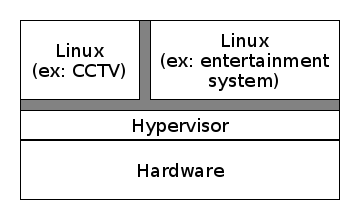
\includegraphics[height=4cm]{figures/figure-1.png}
	\centering
	\caption{
		Two Linux on top of an hypervisor. They run isolated from each other
		and from the hypervisor.
	}
	\label{2-Linux-on-hypervisor-intro}
\end{figure}

Previous work in the PROSPER project achieved \cite{noauthor_prosper:_nodate-1}
to formally verify a simple separation kernel \cite{dam_formal_2013}, which
later resulted into an implementation of a working hypervisor. Then, they
achieved to run both Linux and FreeRTOS on top of it. Finally, they formally
verified memory isolation for virtualized applications
\cite{nemati_trustworthy_2015}. Now, among other projects, the PROSPER team is
working on device virtualization, allowing to give access to hardware devices to
virtualized applications. An interesting example are Network Interface
Controller (NIC) devices, which enable network communication and give the
ability, for example, to communicate thought the Internet.

A formal model of a NIC device has already been produced, on which various
security theorems has been proved \cite{haglund_formal_2016}. These high-level
proofs rely on a set of lower-level lemmas \ref{hol-v-bir-nic-model-simple}.
This layer provides an abstraction over the raw HOL4 model. This is illustrated
in the left-hand side of Figure \ref{hol-v-bir-nic-model-simple}.

In the meantime, the team also developed a framework, TrABin, allowing to search
weakest preconditions for loop-free programs such that a given invariant holds,
directly from the binary code \cite{lindner_trabin:_2019}. This framework
consists of two tools: a transpiler from the actual binary code to a new binary
intermediate representation (BIR), and a weakest precondition prover. While this
kind of transpilers and proof-producing weakest precondition tools already exist
\footnote{see \cite{lindner_trabin:_2019}}, the novelty in this work is that the
transpiler is proof-producing, i.e. it produces a formal proof that both binary
representations are equivalent, under the simulation theory, with respect to the
Instruction Set Architecture (ISA) model. With this method, you no longer need
to trust the transpiler. Figure \ref{trabin-overview} gives an overview of the
TrABin framework\footnote{TrABin works with both ARMv8 and Cortex M0 binary
	programs. Only ARMv8 is showed in Figure \ref{trabin-overview} to save some
space.}.

\begin{figure}[!ht]
	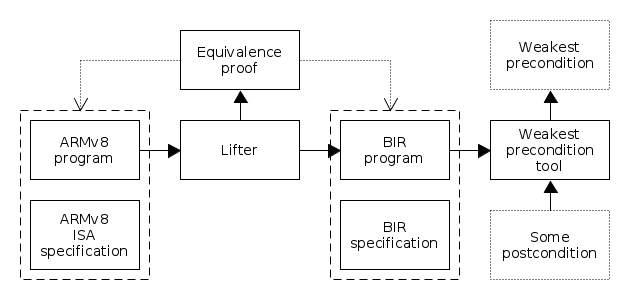
\includegraphics[height=5cm]{figures/trabin-overview.png}
	\centering
	\caption{The TrABin framework. The Lifter generates a BIR program and an
		equivalence proof from an ARMv8 program. The equivalence proof
		established a simulation between the ARMv8 binary program and the
		generated BIR binary program, showing that they have the same behaviour
	with respect to the ARMv8 ISA specification and the BIR specification.}
	\label{trabin-overview}
\end{figure}

The idea of my project is to write a model of a NIC using BIR, then use the
weakest precondition producing tool to prove the same security lemmas than the
HOL4 model. From there, the security properties are implied. Figure
\ref{hol-v-bir-nic-model-simple} gives an overview of this idea: using the
proof-producing weakest precondition tool to bind together a newly written BIR
NIC model and the work done on the formal model.

\begin{figure}[!ht]
	\includegraphics[height=6cm]{figures/figure-2.png}
	\centering
	\caption{HOL4 v. BIR NIC models. The left hand side already exists. This
		project would consist in the dashed elements. The dotted lines represent
	the work to be done during this project.}
	\label{hol-v-bir-nic-model-simple}
\end{figure}

\section{Research Question}

\chapter{Background}

\section{Introducing concepts}

\subsection{Memory sharing between CPU and devices}

Figure \ref{cpu-memory-schema} represents how the CPU and devices can share the
main memory using Direct Memory Access (DMA) \footnote{This schema doesn't
represent caches.}. To read from/write to the main memory, the CPU passes
through the Memory Management Unit (MMU), which is responsible for
virtual/physical address translation. In a nutshell, memory addresses that the
CPU uses are mapped on a virtual address space---each running process having its
own---that are mapped to the actual physical addresses by the MMU. This enables
virtualization and abstraction between processes, which can each have their own
memory spaces in apparent isolation.

Similarly, devices can directly access the main memory using Direct Memory
Access (DMA). This technique enables to offload the CPU from copying each byte
of memory and instead setting the DMA controller to do so. DMA controllers also
give devices direct access to the main memory. While fast and convenient, DMA
creates a whole new range of vulnerabilities. Indeed, if misconfigured, the DMA
controller can give complete access to the main memory to devices, like kernel
private memory, page table or executable memory \cite{schwarz_formal_2014}.

\begin{figure}[!t]
	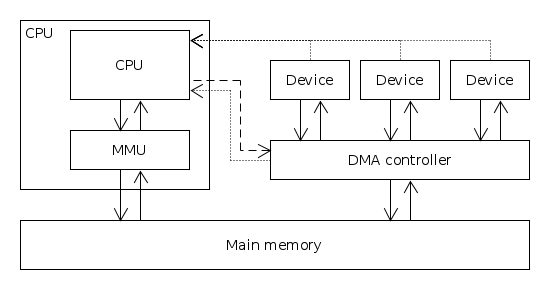
\includegraphics[height=5cm]{figures/cpu-memory-schema.png}
	\centering
	\caption{CPU schema from a memory point of view. The dashed line between the
		CPU and the DMA controller represent the capability of the CPU to send
		commands to the DMA controller through register writes. Dotted lines to
	the CPU represent the ability to raise interrupts.}
	\label{cpu-memory-schema}
\end{figure}

\subsection{Interactive Theorem Proving and HOL4}

Interactive theorem provers are software producing formal proofs, in an
interactive fashion, i.e. a human can step through the proof interactively while
the proof assistant provides some automation (like rewriting of terms,
arithmetic evaluation, integration with external tools like SMT solvers, \dots).
Coq, HOL4 or Isabelle are such tools.

HOL \cite{noauthor_hol_nodate} stands for Higher-Order Logic. It is a
programming environment deeply embedded into the SML programming language
enabling to prove theorems and write proof-producing programs. According to the
official website, and confirmed by the \texttt{examples} directory of the Git
repository \cite{noauthor_canonical_2019}, HOL4 is ``particularly suitable as a
platform for implementing combinations of deduction, execution and property
checking''. Hence, it is well suited to prove properties on hardware.

Several models have been realized of different ARM Instruction Set Architecture
(ISA), such as ARMv3, ARMv4, ARMv7 \cite{noauthor_canonical_2019,
	hutchison_trustworthy_2010} and very recently ARMv8 \cite{armstrong_isa_2019}.
These models enable making proofs directly at the ISA level, avoiding the
necessity to trust the compiler and enabling to formally verify program
behaviours according to the CPU specification.

\subsection{TrABin's Binary Intermediate Representation (BIR)}

TrABin's Binary Intermediate Representation (BIR) \cite{lindner_trabin:_2019},
introduced in the Introduction, is a machine independent binary representation.
It aims to be the simplest possible while still being able to represent all
possible programs. It does so by having a limited syntax---introduced in Table
\ref{bir-syntax}\footnote{for more information, see
	\cite{lindner_trabin:_2019}}---and forbidding implicit side-effects. A statement
can only have explicit state changes and can only affect one variable.

\begin{table}
	\begin{align*}
		pr~    & :=~block^{\ast}                                                             \\
		block~ & :=~(string~|~integer,~bst^{\ast},~cfst)                                     \\
		bst~   & :=~\textbf{assign}~(string, exp)~|~\textbf{assert}~(exp)                    \\
		cfst~  & :=~\textbf{jmp}~(exp)~|~\textbf{cjmp}~(exp,~exp,~exp)                       \\
		exp~   & :=~string~|~integer                                                         \\
		       & ~~~~|~\textbf{ifthenelse}~(exp,~exp,~exp)                                   \\
		       & ~~~~|~\diamond_{u}~exp~|~exp~\diamond_{b}~exp~|~\textbf{var}~string         \\
		       & ~~~~|~\textbf{load}~(exp,~exp,~\tau)~|~\textbf{store}~(exp,~exp,~exp,~\tau) 
	\end{align*}
	\caption{BIR's syntax}
	\label{bir-syntax}
\end{table}

This representation allows to produce proofs more easily that with classical
binary representations, whose design are focused on execution speed rather than
offline analysis. Moreover, BIR is fully specified and doesn't have unspecified
behaviour.

\subsection{Hoare logic and Weakest Preconditions}

According to Wikipedia, ``Hoare logic (also known as Floyd–Hoare logic or Hoare
rules) is a formal system with a set of logical rules for reasoning rigorously
about the correctness of computer programs'' \cite{noauthor_hoare_2019}.

The main tool of Hoare logic is the Hoare triple, which describes how the
execution of a program $C$ affects the state of the execution. They are written
$$\{P\}~C~\{Q\}$$ where $P$ and $Q$ are two predicates, called respectively
precondition and postcondition. $P$ describes the whole set of possible states
as inputs of $C$, and $Q$ describes all the possible states after execution of
$C$.

Here are some simple examples of Hoare triples:
\begin{itemize}
	\item[--] $\{P\}~\varnothing~\{P\}$: an empty program doesn't change the
	      state of the execution.
	\item[--] $\{n\in \mathbb{N} \land odd(n)\}~n:=n+1;~\{even(n)\}$:
	      incrementing the value of an odd integer variable by one makes it even.
\end{itemize}

With Hoare logic comes the idea of weakest precondition: given a program $C$ and
a desired final state $Q$, we want to derive the weakest precondition $P$
allowing to reach a state satisfying $Q$ after executing $C$. Hence, $P$
describes all such states. For example, given the program $x:=x+5$ and the
postcondition $\{x \geq 10\}$ the weakest precondition $P$ is $\{x \geq 5\}$.
This means that all states that satisfy $P$, i.e. all states where $x \geq 5$,
are guaranteed to produce states where $Q$ holds, i.e. where $x \geq 10$.

\section{Related work}

\subsection{Necessity of secure execution platforms}

The PROSPER project isn't the only project focused on high-security execution
platforms. Platforms such that seL4, Microsoft Hyper-V and INTEGRITY Multivisor
are examples of platforms already used in production and providing strong
security properties.

\paragraph{seL4} is a recent L4-based microkernel created in 2006 with the goal
to produce a completely formally verified implementation of a L4 microkernel.
This has been achieved in 2009 \cite{klein_sel4:_2009}. At this time, seL4
consisted of \num{8700} lines of C code and \num{600} lines of assembler. The
implementation of seL4 has been formally from its abstract specification down to
its C implementation. However, the correctness of compilers, assembly code and
hardware has been assumed. PROSPER differs from seL4 by removing the need to
trust the compiler.

\paragraph{Microsoft Hyper-V} is Microsoft's hypervisor, widely used today
within the Microsoft Azure cloud platform. It has been released in 2008. Hyper-V
is a huge codebase, as we can read on VCC's website
\footnote{\url{https://www.microsoft.com/en-us/research/project/vcc-a-verifier-for-concurrent-c/}}:
``Hyper-V consists of about 60 thousand lines of operating system-level C and
x64 assembly code, it is therefore not a trivial target''. Microsoft has put a
lot of work in formal verification\footnotemark of Hyper-V down to machine code
\cite{leinenbach_verifying_2009}. However, they don't appear to include device
drivers in their formal verification.

\footnotetext{Microsoft has several formal verification projects, many of which
	are freely available for non-commercial use:
	\url{https://github.com/Microsoft?q=verifier}}

\paragraph{INTEGRITY Multivisor} is a commercial real-time operating system
developed by Green Hills Software. Although not much information seems to be
publicly available, Green Hills Software has done considerable formal
verification work \cite{richards_modeling_2010}. Multivisor has several
certifications, including, for example, ISO 26262 ASIL D automotive electronics,
NSA-certified secure mobile phones or FAA DO-178B Level A-certified avionics
controlling life-critical functions on passenger and military aircraft
\footnotemark.

\footnotetext{\url{https://ghs.com/products/rtos/integrity_virtualization.html}}

\subsection{Other binary analysis platforms}

For this project, I will use the TrABin framework developed here at KTH
\cite{lindner_trabin:_2019}. However, several other binary analysis platforms
has been created for various purposes, such as formal verification or static
analysis.

\paragraph{} A common characteristic of these platforms is to use an
intermediate representation (IR). IRs are designed to be simpler to use for each
platforms' end purpose. As an example, the TrABin platform has BIR as its
intermediate representation.

\paragraph{Microsoft Boogie} is Microsoft's intermediate verification language.
Boogie is the IR for multiple Microsoft tools, including VCC. Boogie as a tool
can infer some invariants on the given Boogie program and then generate
verification conditions that are passed to an SMT solver \footnotemark.

\footnotetext{\url{https://www.microsoft.com/en-us/research/project/boogie-an-intermediate-verification-language/}}

\paragraph{Valgrind} is a framework for building program supervision tools, such
as memory checkers, cache profilers or data-race detectors
\cite{nethercote_valgrind:_2003}. As its core, Valgrind is a JIT x86-to-x86
compiler, translating binary programs into its IR called UCode. Then,
\textit{skins}---the tools built on the Valgrind framework---are free to
transform and work in the IR to perform several analysis.

\paragraph{LLVM} is a compiler infrastructure which supports a unique
multi-stage optimization system \cite{lattner_llvm:_2002}. LLVM is built around
its IR, LLVM Virtual Instruction Set, which can be described as a strict RISC
architecture with high-level type information. This IR was what made LLVM
successful because it is a pragmatic IR suitable for optimizations at multiple
stages (link-, post-link and run-time) and supporting a wide variety of
transformations.

\paragraph{Mayhem} is a system for automatically finding exploitable bugs in
binary programs and generating working exploits as proof of the discovered
vulnerabilities \cite{cha_unleashing_2012}. It leverages BAP, the Binary
Analysis Platform from Carnegie Mellon University (CMU BAP)
\cite{brumley_bap:_2011}, as its IR. It proceeds by fist JIT-ing each
instruction to the BAP intermediate language (IL) and then performing a custom
symbolic execution.

\paragraph{} There are several other tools, platforms and frameworks, such as
CMU BAP, Angr, LLVM KLEE, and so on, but I cannot review them all here. An
interesting note though is that BIR's design is based upon CMU BAP's IL.

\subsection{Previous work in the team}

In a way, this project consists in bridging Jonas' HOL4 NIC model
\cite{haglund_formal_2016} and Andreas' TrABin framework
\cite{lindner_trabin:_2019}, as shown in Figure
\ref{hol-v-bir-nic-model-simple}.

\chapter{Methods}

\chapter{Results}

\chapter{Discussion}

\chapter{Conclusions}

\printbibliography[heading=bibintoc]

\appendix

\chapter{Something Extra}

\tailmatter % back cover page

\end{document}